% Standalone source of the figure fig:blocks of the Legendre-cell paper: the 36 x 36 single-site matrix
% before and after the change to the partner basis of the cube group.
% Build: pdflatex fig_blocks.tex; the paper includes the PDF. Grey scale only.
% One unit is one unknown. Left: the non-zero pattern of M - K Delta in the natural ordering (four functions
% of nine components each), computed from the closed form at k_S h = 0.1. Right: block diagonal; each irreducible representation Gamma gives an n_Gamma x n_Gamma
% block repeated d_Gamma times (n the multiplicity, d the dimension), even representations first.
\documentclass[border=2pt]{standalone}
% Shared preamble of the standalone figures of the Legendre-cell paper.
\usepackage{amsmath,amssymb,bm}
\usepackage{tikz}
\usetikzlibrary{calc,arrows.meta,decorations.pathreplacing}

\begin{document}
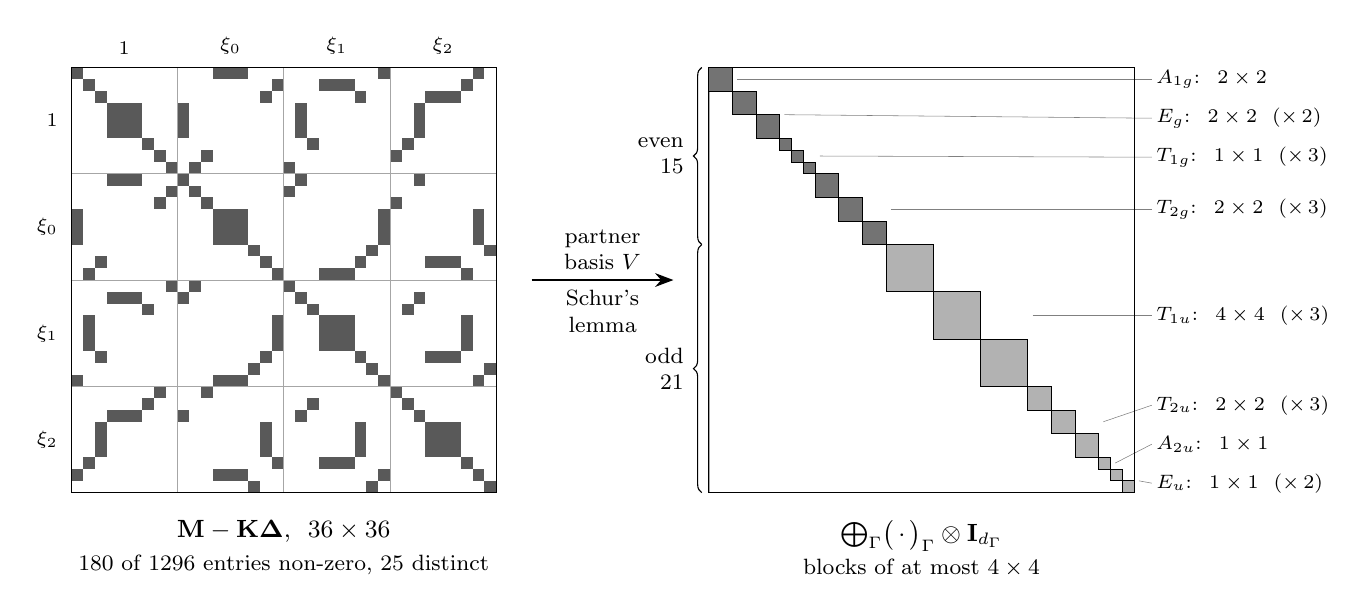
\begin{tikzpicture}[x=0.15cm, y=-0.15cm, >=Stealth, font=\small]
  % ------------------------------------------------------------------ left: the natural ordering
  % the non-zero entries of M - K Delta at k_S h = 0.1 (180 of 1296), from the closed form
  \foreach \j/\i in {0/0,12/0,13/0,14/0,26/0,34/0,1/1,17/1,21/1,22/1,23/1,33/1,2/2,16/2,24/2,30/2,31/2,32/2,3/3,4/3,5/3,9/3,19/3,29/3,3/4,4/4,5/4,9/4,19/4,29/4,3/5,4/5,5/5,9/5,19/5,29/5,6/6,20/6,28/6,7/7,11/7,27/7,8/8,10/8,18/8,3/9,4/9,5/9,9/9,19/9,29/9,8/10,10/10,18/10,7/11,11/11,27/11,0/12,12/12,13/12,14/12,26/12,34/12,0/13,12/13,13/13,14/13,26/13,34/13,0/14,12/14,13/14,14/14,26/14,34/14,15/15,25/15,35/15,2/16,16/16,24/16,30/16,31/16,32/16,1/17,17/17,21/17,22/17,23/17,33/17,8/18,10/18,18/18,3/19,4/19,5/19,9/19,19/19,29/19,6/20,20/20,28/20,1/21,17/21,21/21,22/21,23/21,33/21,1/22,17/22,21/22,22/22,23/22,33/22,1/23,17/23,21/23,22/23,23/23,33/23,2/24,16/24,24/24,30/24,31/24,32/24,15/25,25/25,35/25,0/26,12/26,13/26,14/26,26/26,34/26,7/27,11/27,27/27,6/28,20/28,28/28,3/29,4/29,5/29,9/29,19/29,29/29,2/30,16/30,24/30,30/30,31/30,32/30,2/31,16/31,24/31,30/31,31/31,32/31,2/32,16/32,24/32,30/32,31/32,32/32,1/33,17/33,21/33,22/33,23/33,33/33,0/34,12/34,13/34,14/34,26/34,34/34,15/35,25/35,35/35} {
    \fill[black!65] (\j,\i) rectangle (\j+1,\i+1);
  }
  \foreach \k in {9,18,27} {
    \draw[black!35, very thin] (\k,0) -- (\k,36);
    \draw[black!35, very thin] (0,\k) -- (36,\k);
  }
  \draw (0,0) rectangle (36,36);
  \foreach \a/\lab in {0/1,1/\xi_0,2/\xi_1,3/\xi_2} {
    \node[font=\scriptsize, anchor=south] at (9*\a+4.5,-0.3) {$\lab$};
    \node[font=\scriptsize, anchor=east] at (-0.3,9*\a+4.5) {$\lab$};
  }
  \node[align=center, anchor=north] at (18,37.5)
    {$\mathbf M-\mathbf K\boldsymbol\Delta$, \ $36\times36$\\[1pt]
     \footnotesize $180$ of $1296$ entries non-zero, $25$ distinct};
  % ------------------------------------------------------------------ arrow
  \draw[->, thick] (39,18) -- (51,18)
    node[midway, above, font=\footnotesize, align=center] {partner\\basis $V$}
    node[midway, below, font=\footnotesize, align=center] {Schur's\\lemma};
  % ------------------------------------------------------------------ right: block diagonal
  \begin{scope}[xshift=8.1cm]
    \draw[black!35, very thin] (0,0) rectangle (36,36);
    % name / size n / copies d / shade / first row / label row
    \foreach \name/\n/\d/\shade/\start/\ly in {
        A_{1g}/2/1/55/0/1, E_g/2/2/55/2/4.3, T_{1g}/1/3/55/6/7.6, T_{2g}/2/3/55/9/12,
        T_{1u}/4/3/30/15/21, T_{2u}/2/3/30/27/28.6, A_{2u}/1/1/30/33/31.9, E_u/1/2/30/34/35.2} {
      \foreach \c in {1,...,\d} {
        \pgfmathsetmacro{\lo}{\start + (\c-1)*\n}
        \pgfmathsetmacro{\hi}{\lo + \n}
        \fill[black!\shade] (\lo,\lo) rectangle (\hi,\hi);
        \draw[line width=0.3pt] (\lo,\lo) rectangle (\hi,\hi);
      }
      \pgfmathsetmacro{\mid}{\start + \n*\d/2}
      \pgfmathsetmacro{\edge}{\start + \n*\d}
      \draw[black!50, very thin] (\edge+0.4,\mid) -- (37.5,\ly);
      \node[font=\scriptsize, anchor=west, inner sep=1pt] at (37.6,\ly)
        {$\name$: \ $\n\times\n$\ifnum\d>1{} \ ($\times\,\d$)\fi};
    }
    \draw (0,0) rectangle (36,36);
    \draw[decorate, decoration={brace, amplitude=3pt}] (-0.6,15) -- (-0.6,0)
      node[midway, left=3pt, font=\footnotesize, align=right] {even\\$15$};
    \draw[decorate, decoration={brace, amplitude=3pt}] (-0.6,36) -- (-0.6,15)
      node[midway, left=3pt, font=\footnotesize, align=right] {odd\\$21$};
    \node[align=center, anchor=north] at (18,37.5)
      {$\bigoplus_\Gamma\bigl(\,\cdot\,\bigr)_\Gamma\otimes\mathbf I_{d_\Gamma}$\\[1pt]
       \footnotesize blocks of at most $4\times4$};
  \end{scope}
\end{tikzpicture}
\end{document}
